\documentclass[11pt]{article}
\usepackage{homework}

\classname{364}
\homeworknum{4}

\DeclareMathAlphabet{\mathsfit}{T1}{\sfdefault}{\mddefault}{\sldefault}


\begin{document}

% Environments

\newcommand{\state}[2]{\begin{statement}{#1} #2 \end{statement}}
\newcommand{\prob}[2]{\begin{problem}{#1} #2 \end{problem}}
\newcommand{\subprob}[1]{\begin{subproblem} #1 \end{subproblem}}
\newcommand{\sol}[1]{\begin{solution} #1 \end{solution}}
\newcommand{\fig}[2]{\begin{figure} \centering #2  \label{#1} \end{figure}}

\newcommand{\makebib}{
	\vfill
	\color{black}
	\nocite{*}
	\bibliography{references}{}
	\bibliographystyle{lucas_unsrt}
}
	

% Implication

\newcommand{\qwhere}{\quad \text{where} \quad}
\newcommand{\qimplies}{\quad \implies \quad}
\newcommand{\impliesq}{\implies \quad}



% Brackets

\newcommand{\paren}[1]{\left( #1 \right)}
\newcommand{\brac}[1]{\left[ #1 \right]}
\newcommand{\curly}[1]{\left\{ #1 \right\}}


% Greek

\newcommand{\alp}{\alpha}
\newcommand{\bet}{\beta}
\newcommand{\gam}{\gamma}
\newcommand{\del}{\delta}
\newcommand{\eps}{\epsilon}
\newcommand{\zet}{\zeta}
\newcommand{\tht}{\theta}
\newcommand{\kap}{\kappa}
\newcommand{\lam}{\lambda}
\newcommand{\sig}{\sigma}
\newcommand{\ups}{\upsilon}
\newcommand{\omg}{\omega}

\newcommand{\Gam}{\Gamma}
\newcommand{\Del}{\Delta}
\newcommand{\Tht}{\Theta}
\newcommand{\Lam}{\Lambda}
\newcommand{\Sig}{\Sigma}
\newcommand{\Omg}{\Omega}


% Text

\newcommand{\where}{\text{where }}

% Problem 1

\newcommand{\Hint}{H_\text{int}}
\newcommand{\ddcx}{\dd[3]{x}}
\newcommand{\psib}{\bar{\psi}}

\newcommand{\mh}{m_h}
\newcommand{\mmu}{m_\mu}
\newcommand{\me}{m_e}
\newcommand{\ma}{m_a}

\newcommand{\aexpt}{a_\text{expt.}}
\newcommand{\aQED}{a_\text{QED}}
\renewcommand{\GeV}{\giga\electronvolt}

\newcommand{\gamt}{\gam^5}

\state{}{
	Consider a particle which, as viewed by an observer in an inertial lab, is in a circular orbit in the $(x, y)$ plane with angular velocity $\omg$ and radius $r$.  Suppose that this particle carries a spin angular momentum $\vS$ (treated classically in this problem) which is Fermi-Walker transported.  Compute the time dependence of this angular momentum $\vSt$ where $t$ is the inertial time in the laboratory frame.  Show that in the non-relativistic limit, the complex vector $\Sx + i \Sy$ precesses about the $z$ axis with frequency $\omgT = r^2 \omg^3 / 2$.
}

\sol{
	Since the particle is in a circular orbit in the $xy$ plane, we can write its position in the lab frame as
	\eq{
		\vx = ( t, r \cos(\omg t), r \sin(\omg t), 0 ).
	}
	Then from MCP~(2.7), its velocity is
	\eqn{U}{
		\vU = \dv{\vx}{\tau}
		= \gam ( 1, -r \omg \sin(\omg t), r \omg \cos(\omg t), 0 ),
	}
	since $\ddtau = \ddt / \gam$~\cite[p.~201]{Resnick}.  The particle's acceleration is
	\eq{
		\vaa = \dv{\vU}{\tau}
		= -r \omg^2 \gam^2 ( 0, \cos(\omg t), \sin(\omg t), 0 ).
	}
	The Fermi-Walker transport is, as given by MCP~(24.62),
	\eqn{FW}{
		\nabsU \vS = \vU (\vaa \cdot \vS),
	}
	and we know that the spin vector is always orthogonal to the particle's 4-velocity~\cite[p.~1184]{MCP}.  This means that the spin vector can be written
	\eq{
		\vS = (0, \bS)
	}
	since $\vU \cdot \vS = 0$ is Lorentz invariant, and the spatial components of the particle's velocity are zero in its rest frame.  Moreover, this means
	\eq{
		\nabsU \vS = \dv{\vS}{\tau}
		= \gam \dv{\vS}{t},
	}
	so Eq.~\refeq{FW} can be written
	\eq{
		\dv{\vS}{t} = \frac{1}{\gam} \vU (\vaa \cdot \vS)
		= -\gam r \omg^2 [ \Sx \cos(\omg t) + \Sy \sin(\omg t) ] \vU.
	}
	Feeding in the relevant components of Eq.~\refeq{U}, we have the system of coupled differential equations
	\al{
		\dv{\Sx}{t} &= \gam^2 r^2 \omg^3 \sin(\omg t) [ \Sx \cos(\omg t) + \Sy \sin(\omg t) ], \\
		\dv{\Sy}{t} &= -\gam^2 r^2 \omg^3 \cos(\omg t) [ \Sx \cos(\omg t) + \Sy \sin(\omg t) ],
	}
	or, in matrix form,
	\eqn{sysxy}{
		\dv{t} \mqty[ \Sx \\ \Sy ] = \gam^2 r^2 \omg^3 \mqty[
				\cos(\omg t) \sin(\omg t) & \sin[2](\omg t) \\
				-\cos[2](\omg t) & -\cos(\omg t) \sin(\omg t)
			] \mqty[ \Sx \\ \Sy ].
	}
	% HL FIX THE MINUS 
	To solve the system, we define the polar components of $\vS$ by~\cite[inside cover]{Griffiths}
	\al{
		\Sr &= \Sx \cos(\omg t) + \Sy \sin(\omg t), &
		\Stht &= -\Sx \sin(\omg t) + \Sy \cos(\omg t).
	}
	Then we can transform into these polar coordinates using the matrix~\cite[inside cover]{Griffiths}
	\eqn{sub1}{
		\mqty[ \Sx \\ \Sy ] = \mqty[
				\cos(\omg t) & -\sin(\omg t) \\
				\sin(\omg t) & \cos(\omg t)
			] \mqty[ \Sr \\ \Stht ],
	}
	which implies
	\aln{
		\dv{t} \mqty[ \Sx \\ \Sy ] &= \dv{t} \mqty[
				\cos(\omg t) & -\sin(\omg t) \\
				\sin(\omg t) & \cos(\omg t)
			] \mqty[ \Sr \\ \Stht ] + \mqty[
				\cos(\omg t) & -\sin(\omg t) \\
				\sin(\omg t) & \cos(\omg t)
			] \dv{t} \mqty[ \Sr \\ \Stht ] \\ \notag
		&= -\omg \mqty[
			\sin(\omg t) & \cos(\omg t) \\
			-\cos(\omg t) & \sin(\omg t)
		] \mqty[ \Sr \\ \Stht ] + \mqty[
				\cos(\omg t) & -\sin(\omg t) \\
				\sin(\omg t) & \cos(\omg t)
			] \dv{t} \mqty[ \Sr \\ \Stht ]. \label{sub2}
	}
	Substituting Eqs.~\refeq{sub1} and \refeq{sub2} into Eq.~\refeq{sysxy} yields
	\al{
		-\omg &\mqty[
				\sin(\omg t) & \cos(\omg t) \\
				-\cos(\omg t) & \sin(\omg t)
			] \mqty[ \Sr \\ \Stht ] + \mqty[
				\cos(\omg t) & -\sin(\omg t) \\
				\sin(\omg t) & \cos(\omg t)
			] \dv{t} \mqty[ \Sr \\ \Stht ] \\
		&\hspace{10em} = \gam^2 r^2 \omg^3 \mqty[
				-\cos(\omg t) \sin(\omg t) & -\sin[2](\omg t) \\
				\cos[2](\omg t) & \cos(\omg t) \sin(\omg t)
			] \mqty[
				\cos(\omg t) & -\sin(\omg t) \\
				\sin(\omg t) & \cos(\omg t)
			] \mqty[ \Sr \\ \Stht ] \\
		&\hspace{10em} = \gam^2 r^2 \omg^3 \mqty[
				-\sin(\omg t) & 0 \\
				\cos(\omg t) & 0
			] \mqty[ \Sr \\ \Stht ],
	}
	where the matrix multiplication has been carried out with Mathematica.  This implies
	\al{
		\mqty[
				\cos(\omg t) & -\sin(\omg t) \\
				\sin(\omg t) & \cos(\omg t)
			] \dv{t} \mqty[ \Sr \\ \Stht ]
		&= \paren{ \omg \mqty[
				\sin(\omg t) & \cos(\omg t) \\
				-\cos(\omg t) & \sin(\omg t)
			] + \gam^2 r^2 \omg^3 \mqty[
				-\sin(\omg t) & 0 \\
				\cos(\omg t) & 0
			] } \mqty[ \Sr \\ \Stht ] \\
		&= \omg \mqty[
				(1 - \gam^2 r^2 \omg^2) \sin(\omg t) & \cos(\omg t) \\
				-(1 - \gam^2 r^2 \omg^2) \cos(\omg t) & \sin(\omg t)
			] \mqty[ \Sr \\ \Stht ].
	}
	Multiplying both sides by the inverse of the first matrix, we find
	\eq{
		\dv{t} \mqty[ \Sr \\ \Stht ] = \omg \mqty[
				\cos(\omg t) & \sin(\omg t) \\
				-\sin(\omg t) & \cos(\omg t)
			] \mqty[
				(1 - \gam^2 r^2 \omg^2) \sin(\omg t) & \cos(\omg t) \\
				-(1 - \gam^2 r^2 \omg^2) \cos(\omg t) & \sin(\omg t)
			] \mqty[ \Sr \\ \Stht ]
		= \omg \mqty[
				0 & 1 \\
				\gam^2 r^2 \omg^2 - 1 & 0
			] \mqty[ \Sr \\ \Stht ].
	}
	In other words, we have a system of coupled first-order ODEs:
	\aln{ \label{ODEs}
		\dv{\Sr}{t} &= \omg \Stht, &
		\dv{\Stht}{t} &= \omg (\gam^2 r^2 \omg^2 - 1) \Sr.
	}
%	However, we know that $\Sr(t) = S = \const$, since the magnitude of the spin should not change with time.  Let $\alp \equiv \omg^2 (\gam^2 r^2 \omg^2 - 1)$.  Then, imposing the initial condition $\Stht(0) = 0$,
%	\al{
%		\Sr(t) &= S, &
%		\Stht(t) &= \alp S t.
%	}
%	Now we use Eq.~\refeq{sub1} to transform back to Cartesian components:
%	\al{
%		\Sx(t) &= S \cos(\omg t) - \alp S \sin(\omg t) t
%	}
%	
%	\hl{actually this doesn't make sense}
%
	Differentiating each equation by $t$ once more and substituting, we get a system of uncoupled second-order ODEs with well-known solutions:
	\al{
		\dv[2]{\Sr}{t} &= \omg \dv{\Stht}{t}
		= \omg^2 (\gam^2 r^2 \omg^2 - 1) \Sr, &
		%
		\dv[2]{\Stht}{t} &= \omg (\gam^2 r^2 \omg^2 - 1) \dv{\Sr}{t}
		= \omg^2 (\gam^2 r^2 \omg^2 - 1) \Stht.
	}
	Let $\alp \equiv \omg^2 (\gam^2 r^2 \omg^2 - 1)$.  Then the solutions are~\cite[p.~207]{Swartz}
	\al{
		\Sr(t) &= \Cq \cos(-\alp t) + \Cw \sin(-\alp t), &
		\Stht(t) &= \Dq \cos(-\alp t) + \Dw \sin(-\alp t).
	}
	We transform back into Cartesian components via Eq.~\refeq{sub1}:
	\al{
		\mqty[ \Sx \\ \Sy ] &= \mqty[
				\cos(\omg t) & -\sin(\omg t) \\
				\sin(\omg t) & \cos(\omg t)
			] \mqty[ 
				\Cq \cos(-\alp t) + \Cw \sin(-\alp t) \\
				\Dq \cos(-\alp t) + \Dw \sin(-\alp t)
			] \\
		&= \mqty[
				\cos(\omg t) [ \Cq \cos(-\alp t) + \Cw \sin(-\alp t) ] - \sin(\omg t) [ \Dq \cos(-\alp t) + \Dw \sin(-\alp t) ] \\
				\sin(\omg t) [ \Cq \cos(-\alp t) + \Cw \sin(-\alp t) ] + \cos(\omg t) [ \Dq \cos(-\alp t) + \Dw \sin(-\alp t) ].
			]
	}
	We choose the initial conditions $\Sx(0) = S$, $\Sy(0) = 0$, which give us
	\al{
		\Sx(0) &= S
		= \Cq, &
		%
		\Sy(0) &= 0
		= \Dq.
	}
	Using these results and the initial conditions in Eq.~\refeq{sysxy}, we have
	\eq{
		\left. \dv{t} \mqty[ \Sx \\ \Sy ] \right|_{t = 0} = \gam^2 r^2 \omg^3 \mqty[
				0 & 0 \\
				1 & 0
			] \mqty[
				S \\
				0
			]
		= \gam^2 r^2 \omg^3 \mqty[ 0 \\ S ],
	}
	with
	\eq{
		\left. \dv{t} \mqty[ \Sx \\ \Sy ] \right|_{t = 0} = 
	}
	\hl{but this is getting really gross}
	
	\eq{
		\mqty[ \Sx \\ \Sy ] = \mqty[
				\cos(\omg t) [ S \cos(-\alp t) + \Cw \sin(-\alp t) ] - \Dw \sin(\omg t) \sin(-\alp t) \\
				\sin(\omg t) [ S \cos(-\alp t)  + \Cw \sin(-\alp t) ] + \Dw \cos(\omg t) \sin(-\alp t)
			]
	}
	\eq{
		\mqty[ 0 \\ S ](t = -\pi \alp / 2) = \mqty[
				\Cw \cos(-\pi \omg \alp / 2) - \Dw \sin(-\pi \omg \alp / 2) \\
				\Cw \sin(-\pi \omg \alp / 2) + \Dw \cos(-\pi \omg \alp / 2)
			]
	}
	
	
%	We choose the initial conditions $\Sr(0) = S$ and $\Stht(0) = 0$.  This gives us
%	\al{
%		S &= \Sr(0) = \Cq, &
%		0 &= \Stht(0) = \Dq.
%	}
%	Then by Eq.~\refeq{ODEs},
%	\al{
%		\omg \Dw \sin(-\alp t) &= \dv{\Sr}{t} = \omg \alp [ S \sin(-\alp t) - \Cw \cos(-\alp t) ], \\
%		\omg \alp [ S \cos(-\alp t) + \Cw \sin(-\alp t) ] &= \dv{\Stht}{t} = -\alp \Dw \cos(-\alp t)
%	}
}





\clearpage
\newcommand{\Fab}{F^{\alp \bet}}
\newcommand{\Ua}{U^\alp}
\newcommand{\Usa}{U_\alp}
\newcommand{\Ub}{U^\bet}
\newcommand{\Xa}{X^\alp}
\newcommand{\Xsa}{X_\alp}
\newcommand{\Xb}{X^\bet}
\newcommand{\xap}{x^\alp_p}
\newcommand{\xaq}{x^\alp_q}

\begin{statement}{(Jackson 11.17)}
	The electric and magnetic fields \refeq{fields} of a charge in uniform motion can be obtained from Coulomb's law in the charge's rest frame and the fact that the field strength $\Fab$ is an antisymmetric tensor of rank 2 without considering \emph{explicitly} the Lorentz transformation.  The idea is the following.  For a charge in uniform motion the only relevant variables are the charge's 4-velocity $\Ua$ and the relative coordinate $\Xa = \xap - \xaq$, where $\xap$ and $\xaq$ are the 4-vector coordinates of the observation point and the charge, respectively.  The only antisymmetric tensor that can be formed is $(\Xa \Ub - \Xb \Ua)$.  Thus the electromagnetic field $\Fab$ must be this tensor multiplied by some scalar function of the possible scalar products, $\Xsa \Xa$, $\Xsa \Ua$, $\Usa \Ua$.
\end{statement}

\newcommand{\vbb}{\vb{b}}
\newcommand{\vv}{\vb{v}}
\newcommand{\Eq}{E_1}
\newcommand{\Ew}{E_2}
\newcommand{\Ee}{E_3}
\newcommand{\Bq}{B_1}
\newcommand{\Bw}{B_2}
\newcommand{\Be}{B_3}

\newcommand{\xsq}{x^1}


\begin{figure} \centering
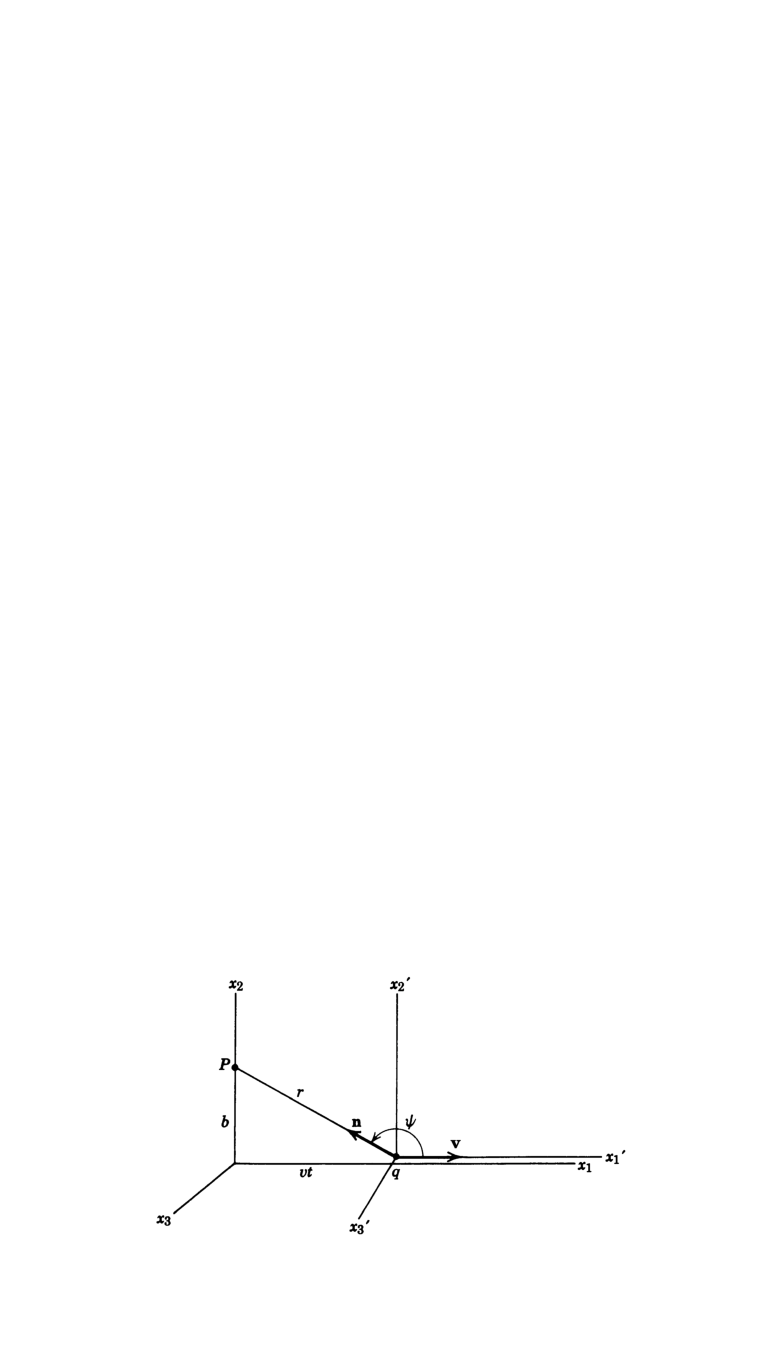
\includegraphics{11-8}
\caption{(Jackson Fig.~11.8) Particle of charge $q$ moving at constant velocity $\vv$ passes an observation point $P$ at impact parameter $b$.}
\label{11.8}
\end{figure}

\begin{problem} \label{2.a}
	For the geometry of Fig.~\ref{11.8} the coordinates of $P$ and $q$ at a common time in $K$ can be written $\xap = (ct, \vbb)$, $\xaq = (ct, \vv t)$, with $\vbb \vdot \vv = 0$.  By considering the general form of $\Fab$ in the rest frame of the charge, show that
	\beqn \label{show2.a}
		\Fab = \frac{q}{c} \frac{\Xa \Ub - \Xb \Ua}{[(\Usa \Xa / c)^2 - \Xsa \Xa]^{3/2}}.
	\eeqn
	Verify that this yields the expressions
	\begin{align} \label{fields}
		\Eq &= \Eq' = -\frac{q \gam v t}{(b^2 + \gam^2 v^2 t^2)^{3/2}}, &
		\Ew &= \gam \Ew' = \frac{\gam q b}{(b^2 + \gam^2 v^2 t^2)^{3/2}}, &
		\Be &= \gam \bet \Ew' = \bet \Ew,
	\end{align}
	with all other components vanishing, in the inertial frame $K$.
\end{problem}


\newcommand{\Fmat}{\mqty[	0 & -\Eq & -\Ew & -\Ee \\
						\Eq & 0 & -\Be & \Bw \\
						\Ew & \Be & 0 & -\Bq \\
						\Ee & -\Bw & \Bq & 0 ]}
\newcommand{\Fpab}{{F'}^{\alp\bet}}
\newcommand{\rp}{{r'}}
\newcommand{\tLam}{\tilde{\Lam}}
\newcommand{\Lammat}{\mqty[\gam & \gam \beta & 0 & 0 \\	
						\gam \beta & \gam & 0 & 0 \\
						0 & 0 & 1 & 0 \\
						0 & 0 & 0 & 1 ]}

\begin{solution}
	From Jackson~(11.137),
	\beqn \label{F}
		\Fab = \Fmat,
	\eeqn
	and from the equation immediately preceding Jackson~(11.151),
	\begin{align*}
		\Eq' &= -\frac{q v t'}{\rp^3}, &
		\Ew' &= \frac{q b}{\rp^3}, &
		\Ee' &= 0, &
		\Bq' &= 0, &
		\Bw' &= 0, &
		\Be' &= 0,
	\end{align*}
	in the rest frame of the charge for the geometry in Fig.~\ref{1}.  Here, $r' = \sqrt{b^2 + v^2 {t'}^2}$.  Then, in $K'$,
	\beqn \label{thing2.1b}
		\Fpab = \frac{q}{(b^2 + v^2 {t'}^2)^{3/2}}
			\mqty[0 & v t' & -b & 0 \\
				-v t' & 0 & 0 & 0 \\
				b & 0 & 0 & 0 \\
				0 & 0 & 0 & 0 ].
	\eeqn
	Now we will boost into the frame $K$.  From Jackson~(11.147), $F' = \Lam F \tLam$, although we need $F = \Lam F' \tLam$, where we boost in the direction opposite the particle's motion.  According to Jackson~(11.113), the Lorentz boost in the $-x'$ direction is
	\beqn \label{Lam2}
		\Lam = \Lammat.
	\eeqn
	Then
	\begin{align*}
		\Fab &= \frac{q}{(b^2 + v^2 {t'}^2)^{3/2}} \Lammat
			\mqty[ 0 & v t' & -b & 0 \\
				-v t' & 0 & 0 & 0 \\
				b & 0 & 0 & 0 \\
				0 & 0 & 0 & 0 ]
			\Lammat \\
		&= \frac{q}{(b^2 + v^2 {t'}^2)^{3/2}}
			\mqty[ -\gam \bet v t' & \gam v t' & -\gam b & 0 \\
				-\gam v t' & \gam \bet v t' & -\gam \bet b & 0 \\
				b & 0 & 0 & 0 \\
				0 & 0 & 0 & 0 ]
			\Lammat
		= \frac{q}{(b^2 + v^2 {t'}^2)^{3/2}}
			\mqty[ 0 & v t' & -\gam b & 0 \\
				-v t' & 0 & -\gam \bet b & 0 \\
				\gam b & \gam \bet b & 0 & 0 \\
				0 & 0 & 0 & 1 ].
	\end{align*}
	From \refeq{lorentz}, $t' = \gam t$ since $x = 0$.  Finally,
	\beqn \label{thing2.1}
		\Fab = \frac{\gam q}{(b^2 + \gam^2 v^2 t^2)^{3/2}} 
			\mqty[0 & v t & -b & 0 \\
				-v t & 0 & -v b / c & 0 \\
				b & v b / c & 0 & 0 \\
				0 & 0 & 0 & 0 ].
	\eeqn
	
	Now we will begin from \refeq{show2.a} and find $\Fab$ directly in $K$.  In accordance with Fig.~\ref{11.8},
	\begin{align*}
		\Xa &= (0, \vbb - \vv t) = (0, -v t, b, 0), &
		\Ua &= \gam (c, \vv) = \gam (c, v, 0, 0),
	\end{align*}
	and so
	\beq
		\Xa \Ub - \Xb \Ua = \gam
			\mqty[ 0 & 0 & 0 & 0 \\
				-c v t & -v^2 t & 0 & 0 \\
				c b & v b & 0 & 0 \\
				0 & 0 & 0 & 0 ]
		- \gam
			\mqty[ 0 & -c v t & c b & 0 \\
				0 & -v^2 t & v b & 0 \\
				0 & 0 & 0 & 0 \\
				0 & 0 & 0 & 0 ]
		= \gam
			\mqty[0 & c v t & - c b & 0 \\
				-c v t & 0 & -v b & 0 \\
				c b & v b & 0 & 0 \\
				0 & 0 & 0 & 0 ].
	\eeq
	Additionally,
	\begin{align*}
		\Usa \Xa &= \gam \mqty[ c & -v & 0 & 0 ] \mqty[ 0 \\ -v t \\ b \\ 0 ]
		= \gam v^2 t, &
		\Xsa \Xa &= \mqty[ 0 & vt & -b & 0 ] \mqty[ 0 \\ -v t \\ b \\ 0 ]
		= -v^2 t^2 - b^2.
	\end{align*}
	Then, applying \refeq{show2.a},
	\beq
		\Fab = \frac{\gam q}{(\gam^2 v^4 t^2 / c^2 + v^2 t^2 + b^2)^{3/2}}
			\mqty[0 & v t & -b & 0 \\
				-v t & 0 & -v b / c & 0 \\
				b & v b / c & 0 & 0 \\
				0 & 0 & 0 & 0 ].
	\eeq
	Note that
	\beq
		v^2 t^2 + \frac{\gam^2 v^4 t^2}{c^2} = v^2 t^2 \left( 1 + \gam^2 \frac{v^2}{c^2} \right)
		= v^2 t^2 \left( 1 + \frac{\bet^2}{1 - \bet^2} \right)
		= v^2 t^2 \frac{1 - \bet^2 + \bet^2}{1 - \bet^2}
		= \gam^2 v^2 t^2,
	\eeq
	so we have again arrived at \refeq{thing2.1}.  Thus, we have proven \refeq{show2.a}.
	
	In addition, comparing \refeq{thing2.1} with \refeq{F}, we see that
	\begin{align*}
		\Eq &= -\frac{q \gam v t}{(b^2 + \gam^2 v^2 t^2)^{3/2}}, &
		\Ew &= \frac{\gam q b}{(b^2 + \gam^2 v^2 t^2)^{3/2}}, &
		\Be &= \frac{\gam \bet q b}{(b^2 + \gam^2 v^2 t^2)^{3/2}} = \bet \Ew.
	\end{align*}
	Comparing \refeq{thing2.1b} with \refeq{F} as well, and making the substitution $t' = \gam t$, yields
	\begin{align*}
		\Eq' &= -\frac{q \gam v t}{(b^2 + \gam^2 v^2 t^2)^{3/2}}, &
		\Ew' &= \frac{q b}{(b^2 + \gam^2 v^2 t^2)^{3/2}},
	\end{align*}
	so we have also verified \refeq{fields}. \qed
\end{solution}


\newcommand{\xpap}{{x'}^\alp_p}
\newcommand{\xpaq}{{x'}^\alp_q}
\newcommand{\Ya}{Y^\alp}
\newcommand{\Ysa}{Y_\alp}
\newcommand{\Yb}{Y^\bet}
\newcommand{\Ypa}{{Y'}^\alp}

\begin{problem}
	Repeat the calculation, using as the starting point the common-time coordinates in the rest frame, ${\xpap = (ct', \vbb - \vv t')}$ and $\xpaq = (ct', 0)$.  Show that
	\beqn \label{show2.b}
		\Fab = \frac{q}{c} \frac{\Ya \Ub - \Yb \Ua}{(- \Ysa \Ya)^{3/2}},
	\eeqn
	where $\Ypa = \xpap - \xpaq$.  Verify that the fields are the same as in \ref{2.a}.  Note that to obtain the results of \refeq{fields} it is necessary to use the time $t$ of the observation point $P$ in $K$ as the time parameter.
\end{problem}

\newcommand{\Ypsa}{{Y'}_\alp}
\newcommand{\Ypb}{{Y'}^\bet}
\newcommand{\Upa}{{U'}^\alp}
\newcommand{\Upb}{{U'}^\bet}
\newcommand{\vo}{\mathbf{0}}
\newcommand{\tp}{{t'}}

\begin{solution}
	Firstly, note that
	\begin{align*}
		\Ypa &= (0, \vbb - \vv t') = (0, -v t', b, 0), &
		\Upa &= (c, \vo) = (c, 0, 0, 0),
	\end{align*}
	Then
	\beq
		\Ypa \Upb - \Ypb \Upa = c
			\mqty[ 0 & 0 & 0 & 0 \\
				-v t' & 0 & 0 & 0 \\
				b & 0 & 0 & 0 \\
				0 & 0 & 0 & 0 ]
		- c
			\mqty[ 0 & -v t' & b & 0 \\
				0 & 0 & 0 & 0 \\
				0 & 0 & 0 & 0 \\
				0 & 0 & 0 & 0 ]
		= c
			\mqty[ 0 & v t' & -b & 0 \\
				-v t' & 0 & 0 & 0 \\
				b & 0 & 0 & 0 \\
				0 & 0 & 0 & 0 ],
	\eeq
	and
	\beq
		\Ypsa \Ypa = \mqty[ 0 & v t' & -b & 0 ] \mqty[ 0 \\ -v t' \\ b \\ 0 ] = -v^2 \tp^2 - b^2,
	\eeq
	so, from \refeq{show2.b}, in $K'$ we have
	\beq
		\Fpab = \frac{q}{(b^2 + v^2 \tp^2)^{3/2}}
			\mqty[ 0 & v t' & -b & 0 \\
				-v t' & 0 & 0 & 0 \\
				b & 0 & 0 & 0 \\
				0 & 0 & 0 & 0 ],
	\eeq
	which is identical to \refeq{thing2.1b}.  We know that boosting into $K$ yields \refeq{thing2.1}.
	
	Now we will find $\Fab$ directly in $K$ by boosting $\Ypa$ and $\Upa$.  From Jackson~(11.84), $x' = \Lam x$ (where $x$ represents $x^\alp$), and we once again use $\Lam$ given by \refeq{Lam2} to perform $x = \Lam x'$.  We obtain
	\begin{align*}
		Y &= \Lam Y'
		= \Lammat \mqty[ 0 \\ -v t' \\ b \\ 0]
		= \mqty[ -\gam \bet v t' \\ -\gam v t' \\ b \\ 0 ], &
		U &= \Lam U'
		= \Lammat \mqty[ c \\ 0 \\ 0 \\ 0 ]
		= \gam c \mqty[ 1 \\ \bet \\ 0 \\ 0 ].
	\end{align*}
	Then
	\beq
		\Ya \Ub - \Yb \Ua = \gam c
			\mqty[ -\gam \bet v t' & -\gam \bet^2 v t' & 0 & 0 \\
				-\gam v t' & -\gam \bet v t' & 0 & 0 \\
				b & \bet b & 0 & 0 \\
				0 & 0 & 0 & 0 ]
			- \gam c
			\mqty[ -\gam \bet v t' & -\gam v t' & b & 0 \\
				-\gam \bet^2 v t' & -\gam \bet v t' & \bet b & 0 \\
				0 & 0 & 0 & 0 \\
				0 & 0 & 0 & 0 ]
		= c
			\mqty[ 0 & v t' & -\gam b & 0 \\
				-v t' & 0 & -\gam \bet b & 0 \\
				\gam b & \gam \bet b & 0 & 0 \\
				0 & 0 & 0 & 0 ],
	\eeq
	and
	\beq
		\Ysa \Ya = \mqty[ -\gam \bet v t' & \gam v t' & -b & 0] \mqty[ -\gam \bet v t' \\ -\gam v t' \\ b \\ 0 ]
		= \gam^2 \bet^2 v^2 \tp^2 - \gam^2 v^2 \tp^2 - b^2
		= -v^2 \tp^2 - b^2.
	\eeq
	Making these substitutions into \refeq{show2.b}, and using $t' = \gam t$,
	\beq
		\Fab = \frac{q}{(b^2 + v^2 \tp^2)^{3/2}}
			\mqty[ 0 & v t' & -\gam b & 0 \\
				-v t' & 0 & -\gam v b / c & 0 \\
				\gam b & \gam v b / c & 0 & 0 \\
				0 & 0 & 0 & 0 ]
		= \frac{\gam q}{(b^2 + \gam^2 v^2 t^2)^{3/2}}
			\mqty[ 0 & v t & -b & 0 \\
				-v t & 0 & -v b / c & 0 \\
				b & v b / c & 0 & 0 \\
				0 & 0 & 0 & 0 ],
	\eeq
	which is identical to \refeq{thing2.1}, and therefore gives the fields from \refeq{fields} as in \ref{2.a}.  Thus, we have proven \refeq{show2.b}. \qed
\end{solution}


\newcommand{\Za}{Z^\alp}
\newcommand{\Zsa}{Z_\alp}
\newcommand{\Zb}{Z^\bet}
\newcommand{\vbet}{\boldsymbol{\beta}}

\begin{problem}
	Finally, consider the coordinate $\xap = (ct, \vbb)$ and the ``retarded-time'' coordinate $\xaq = [ct - R, \vbet(ct - R)]$ where $R$ is the distance between $P$ and $q$ at the retarded time.  Define the difference as $\Za = [R, \vbb - \vbet(ct - R)]$.  Show that in terms of $\Za$ and $\Ua$ the field is
	\beqn \label{show2.c}
		\Fab = \frac{q}{c} \frac{\Za \Ub - \Zb \Ua}{(\Usa \Za / c)^3}.
	\eeqn
\end{problem}
\vfix

\begin{solution}
	Referring to Fig~\ref{11.8},
	\begin{align*}
		\Za &= (R, \vbb - \vv t + \vv R / c) = [R, -v (t - R / c), b, 0], &
		\Ua &= \gam (c, \vv) = \gam (c, v, 0, 0).
	\end{align*}
	Then
	\begin{align*}
		\Za\Ub - \Zb \Ua &= \gam
			\mqty[c R & R v & 0 & 0 \\
				-v (c t - R) & -v^2 (t - R / c) & 0 & 0 \\
				c b & b v & 0 & 0 \\
				0 & 0 & 0 & 0 ]
			- \gam
			\mqty[ c R & -v (c t - R) & c b & 0 \\
				R v & -v^2 (t - R / c) & b v & 0 \\
				0 & 0 & 0 & 0 \\
				0 & 0 & 0 & 0 ] \\
		&= \gam c
			\mqty[0 & v t & -b & 0 \\
				-v t & 0 & -v b / c & 0 \\
				b & v b / c & 0 & 0 \\
				0 & 0 & 0 & 0 ],
	\end{align*}
	and
	\beq
		\Usa \Za = \gam \mqty[ c & -v & 0 & 0 ] \mqty[ R \\ -v (t - R / c) \\ b \\ 0 ]
		= \gam cR + \gam v^2(t - R/c),
	\eeq
	so
	\beq
		\frac{\Usa \Za}{c} = \gam R + \gam \bet^2 c t - \gam \bet^2 R
		= (1 - \bet^2) \gam R + \gam \bet^2 c t
		= \frac{R}{\gam} + \gam \bet^2 c t.
	\eeq
	
	Note that $\xap$ and $\xaq$, as they are defined here, have lightlike separation since $R / c$ is, by definition, the time it takes light to travel from $\xaq$ to $\xap$.  Then
	\beq
		0 = \Zsa \Za
		= \mqty[ R & v (t - R / c) & -b & 0 ] \mqty[ R \\ -v (t - R / c) \\ b \\ 0 ]
		= R^2 - v^2 (t - R / c)^2 - b^2,
	\eeq
	which implies
	\beq
		R^2 = b^2 + v^2 (t - R / c)^2.
	\eeq
	This is corroborated by the geometry of Fig.~\ref{11.8}, since $t - R / c$ is the retarded time.  Then, referring to the denominator of \refeq{thing2.1}, we find
	\begin{align*}
		b^2 + \gam^2 v^2 t^2 &= R^2 - v^2 (t - R / c)^2 + \gam^2 v^2 t^2
		= R^2 - \bet^2  (c^2 t^2 - 2 R c t + R^2) + \gam^2 \bet^2 c^2 t^2 \\
		&= (1 - \bet^2) R^2 + 2 R \bet^2 c t + (\gam^2 - 1) \bet^2 c^2 t^2
		= \frac{R^2}{\gam^2} + 2 R \bet^2 c t + \gam^2 \bet^4 c^2 t^2
		= \left( \frac{R}{\gam} + \gam \bet^2 c t \right)^2 \\
		&= \left( \frac{\Usa \Za}{c} \right)^2.
	\end{align*}
	In summary, we have found
	\beq
		\Fab = \frac{\gam q}{(b^2 + \gam^2 v^2 t^2)^{3/2}}
			\mqty[0 & v t & -b & 0 \\
				-v t & 0 & -v b / c & 0 \\
				b & v b / c & 0 & 0 \\
				0 & 0 & 0 & 0 ],
	\eeq
	which is identical to \refeq{thing2.1}.  Thus, we have proven \refeq{show2.c}. \qed
\end{solution}





\clearpage
\state{Rigidly rotating disk~(MCP 24.17)}{
	Consider a thin disk with radius $R$ at $z = 0$ in a Lorentz reference frame.  The disk rotates rigidly with angular velocity $\Omg$.  In the early years of special relativity there was much confusion over the geometry of the disk: In the inertial frame it has physical radius (proper distance from center to edge) $R$ and physical circumference $\sC = 2\pi R$.  But Lorentz contraction dictates that, as measured on the disk, the circumference should be $\sqrt{1 - v^2} \sC$ (with $v = \Omg R$), and the physical radius, $R$, should be unchanged.  This seemed weird.  How could an obviously flat disk in spacetime have a curved, non-Euclidean geometry, with physical circumference divided by physical radius smaller than $2\pi$?  In this exercise you will explore this issue.
}

\prob{
	Consider a family of observers who ride on the edge of the disk.  Construct a circular curve, orthogonal to their world lines, that travels around the disk (at $\sqrt{x^2 + y^2} = R$).  This curve can be thought of as lying in a 3-surface of constant time $\xoh$ of the observers' proper reference frames.  Show that it spirals upward in a Lorentz-frame spacetime diagram, so it cannot close on itself after traveling around the disk.  Thus the 3-planes, orthogonal to the observers' world lines at the edge of the disk, cannot mesh globally to form global 3-planes.
}

\sol{
	We can write the position of an observer in an inertial reference frame as
	\eq{
		\vx = ( t, R \cos(\Omg t), R \sin(\Omg t), 0 ).
	}
	Then the velocity of the observer, which is tangent to his/her worldline, is
	\eq{
		\vuu = \dv{\vx}{\tau}
		= \gam ( 1, -R \Omg \sin(\Omg t), R \Omg \cos(\Omg t), 0 ).
	}
	By inspection, a vector orthogonal to this velocity is
	\eq{
		\vv = \gam ( R^2 \Omg^2, -R \Omg \sin(\Omg t), R \Omg \cos(\Omg t), 0 )
		= \dv{\vy}{\tau},
	}
	where $\vy$ traces out the curve orthogonal to the world line.  It is given by
	\eq{
		\vy = ( R^2 \Omg^2 t , R \cos(\Omg t), R \sin(\Omg t), 0 ).
	}
	We note that $\vy$ traces out a helix in a Lorentz-frame spacetime diagram.  Thus, it cannot close on itself after traveling around the disk. \qed
}



\prob{
	Next, consider a 2-dimensional family of observers who ride on the surface of the rotating disk.  Show that at each radius $\sqrt{x^2 + y^2} = \const$, the constant-radius curve that is orthogonal to their world lines spirals upward in spacetime with a different slope.  Show that this means that even locally, the 3-planes orthogonal to each of their world lines cannot mesh to form larger 3-planes---thus there does not reside in spacetime any 3-surface orthogonal to these observers' world lines.  There is no 3-surface that has the claimed non-Euclidean geometry.
}

\sol{
	For a given radius $r = \sqrt{x^2 + y^2}$, the constant-radius curve that is orthogonal to the worldline is given by
	\eq{
		\vy = ( r^2 \Omg^2 t, -r \Omg \sin(\Omg t), r \Omg \cos(\Omg t), 0 ).
	}
	The slope at which this curve spirals upward in the spacetime diagram is $r^2 \Omg^2 / r = r \Omg^2$~\cite{Helix}, which has a linear dependence on the radius.  Thus, the slope is different for different radii. \qed
	
	\hl{what about the meshing?}
}






\clearpage
\state{Constant of geodesic motion in a spacetime with symmetry~(MCP 25.4)}{\hfix}

\prob{ \label{4a}
	Suppose that in some coordinate system the metric coefficients are independent of some specific coordinate $\xA$: $\sgsabA = 0$ (e.g., in spherical polar coordinates $\{ t, r, \tht, \phi \}$ in flat spacetime $\sgsabphi = 0$, so we could set $\xA = \phi$).  Show that
	\eq{
		\psA \equiv \vp \cdot \pdv{\xA}
	}
	is a constant of the motion for a freely moving particle [$\psp = (\text{conserved $z$~component of angular momentum})$] in the above, spherically symmetric example.]
	
	Hint: Show that the geodesic equation can be written in the form
	\eq{
		\dv{\psa}{\zet} - \Gamsman \pmu \pnu = 0,
	}
	where $\Gamsman$ is the covariant connection of Eqs.~(24.38c), (24.38d) with $\csabg = 0$, because we are using a coordinate basis.
%	
%	Note the analogy of the constant of motion $\psA$ with Hamiltonian mechanics; there, if the Hamiltonian is independent of $\xA$, then the generalized momentum $\psA$ is conserved; here, if the metric coefficients are independent of $\xA$, then the covariant component $\psA$ of the momentum is conserved.
}

\sol{
	The general form of the geodesic equation is given by MCP~(25.11c),
	\eqn{geodesic}{
		\nabsvp \vp = 0.
	}
	Dotting both sides by $\vp$ yields
	\eq{
		0 = \vp \cdot \nabsvp \vp
		\qimplies
		0 = \pmu \nabsm \psa.
	}
	The covariant components of the gradient are given by (24.36), $A_{\alp; \bet} = A_{\alp, \bet} - \Gam^\mu{}_{\alp \bet} A_\mu$, where $A_{\alp, \bet} = \ptsb A_\alp$ and $A_{\alp; \bet} = \nabsb A_\alp$.  Applying this, we have
	\eqn{thing4a}{
		0 = \pmu (p_{\alp, \mu} - \Gamgsam \psg)
		= \pmu \ptsm \psa - \Gamgsam \pmu \psg.
	}
	Using $\vp / m = \dv*{\vx}{\tau}$ and $\tau = m \zeta$~\cite[p.~1202]{MCP}, we can rewrite the first term of Eq.~\refeq{thing4a}:
	\eq{
		\pmu \ptsm \psa = m \dv{\xm}{\tau} \ptsm \psa
		= m \dv{\psa}{\tau}
		= \dv{\psa}{\zet}.
	}
	For the second term of Eq.~\refeq{thing4a}, we multiply by the metric $\sgsba$ as in (24.38d), $\Gam^\mu{}_{\bet \gam} = \sg^{\mu \alp} \Gam_{\alp \bet \gam}$.  Then we have
	\eq{
		\Gamgsam \pmu \psg = \sggn \Gamsnam \pmu \psg
		= \Gamsnam \pmu \pnu
		= \Gamsman \pmu \pnu,
	}
	where in the final step we have relabeled indices.  Thus we can write Eq.~\refeq{thing4a} as
	\eqn{thing4a2}{
		\dv{\psa}{\zet} - \Gamsman \pmu \pnu = 0,
	}
	as recommended.
	
	Now we apply (24.38c); in a coordinate basis, it reduces to
	\eqn{Gam}{
		\Gamsabg = \frac{1}{2} (\sgsabg + \sgsagb - \sgsbga).
	}
	Then for the second term of Eq.~\refeq{thing4a2}, we can write
	\al{
		\Gamsman \pmu \pnu &= \frac{1}{2} (\sg_{\mu \alp, \nu} + \sg_{\mu \nu, \alp} - \sg_{\alp \nu, \mu} ) \pmu \pnu \\
		&= \frac{1}{2} (\sg_{\nu \alp, \mu} + \sg_{\nu \mu, \alp} - \sg_{\alp \mu, \nu} ) \pmu \pnu \\
		&= \frac{1}{2} (\sg_{\alp \nu, \mu} + \sg_{\mu \nu, \alp} - \sg_{\mu \alp, \nu} ) \pmu \pnu \\
		&= \frac{1}{2} \sgsmna \pmu \pnu,
	}
	where we have again relabeled indices, and also used the symmetry of the metric.  Then for Eq.~\refeq{thing4a2}, we have
	\eq{
		\dv{\psa}{\zet} = \frac{1}{2} \sgsmna \pmu \pnu.
	}
	Therefore when $\alp = A$,
	\eq{
		\dv{\psA}{\zet} = \frac{1}{2} \sgsmnA \pmu \pnu = 0
		\qimplies
		\dv{\psA}{\tau} = 0
		\qimplies
		\psA = \const,
	}
	as we wanted to show~\cite[pp.~134--135]{Carroll}. \qed
}



\prob{
	As an example, consider a particle moving freely through a time-independent, Newtonian gravitational field.  In Ex.~25.18, we learn that such a gravitational field can be described in the language of general relativity by the spacetime metric
	\eq{
		\dds^2 = -(1 + 2 \Phi) \ddt^2 + (\delsjk + \hsjk) \ddxj \ddxk,
	}
	where $\Phi(x, y, z)$ is the time-independent Newtonian potential, and $\hsjk$ are contributions to the metric that are independent of the time coordinate $t$ and have magnitude of order $\abs{\Phi}$.  That the gravitational field is weak means $\abs{\Phi} \ll 1$% (or, in conventional units, $\abs{\Phi / c^2} \ll 1$)
	.  The coordinates being used are Lorentz, aside from tiny corrections of order $\abs{\Phi}$, and as this exercise and Ex.~25.18 show, they coincide with the coordinates of the Newtonian theory of gravity.  Suppose that the particle has velocity $\vj \equiv \dv*{\xj}{t}$ through this coordinate system that is $\lesssim \abs{\Phi}^{1/2}$ and thus is small compared to the speed of light.  Because the metric is independent of the time coordinate $t$, the component $\pst$ of the particle's 4-momentum must be conserved along its world line.  Since throughout physics, the conserved quantity associated with time-translation invariance is always the energy, we expect that $\pst$, when evaluated accurate to first order in $\abs{\Phi}$, must be equal to the particle's conserved Newtonian energy, $E = m \Phi + m \vj \vk \delsjk / 2$, aside from some multiplicative and additive constants.  Show that this, indeed, is true, and evaluate the constants.
}





\clearpage
\state{Killing vector field~(MCP 25.5)}{
	A \emph{Killing vector field} is a coordinate-independent tool for exhibiting symmetries of the metric.  It is any vector field $\vxi$ that satisfies
	\eqn{show5}{
		\xisascb + \xisbsca = 0
	}
	(i.e., any vector field whose symmetrized gradient vanishes).
}

\prob{ \label{5a}
	Let $\vxi$ be a vector field that might or might not be Killing.  Show, by construction, that it is possible to introduce a coordinate system in which $\vxi = \pdv*{\xA}$ for some coordinate $\xA$.
}

\sol{
	We know that a single vector can be defined as an arrow residing in the tangent space to some curved manifold at a point we call $\cP$.  We can imagine a projection of $\vxi$ onto the manifold; such a projection is a curve on the manifold.  We may choose the direction of this curve as a coordinate of the manifold and call it $\xA$.  The curve itself we call $\cP(\xA)$.  Then, by construction, $\vxi$ is tangent to $\cP(\xA)$.  This means that $\vxi$ must be the directional derivative along $\cP(\xA)$, which is $\pdv*{\xA}$~\cite[pp.~1166--1167]{MCP}.
	
	For a vector field, the situation is slightly more complex.  Any given manifold can be described by a set of curves that are nonintersecting and which fill the manifold completely.  (Imagine a contour plot of some surface with an infinite number of contours; the contours are the curves in question.)  These are called ``integral curves''~\cite[p.~430]{Carroll}.  Any two integral curves that are arbitrarily close to one another run in the same direction.  So we can use this direction to define a coordinate system with the coordinate $\xA$ along the direction of the integral curves.  Any point $\cP$ on the manifold has an integral curve running through it, and we call this curve $\cP(\xA)$.  The vector tangent to the manifold at $\cP$ is $\pdv*{\xA}$~\cite[pp.~1166--1167]{MCP}.  Since this is true at any point $\cP$ on the manifold, the set of vectors tangent to all such integral curves make up a vector field.  Running this logic in reverse, then, it is possible to start with an arbitrary vector field $\vxi$ and construct a coordinate system in which $\vxi = \pdv*{\xA}$~\cite[p.~430]{Carroll}. \qed
}



\prob{
	Show that in the coordinate system of \ref{5a} the symmetrized gradient of $\vxi$ is $\xisascb + \xisbsca = \pdv*{\sgsab}{\xA}$.  From this infer that a vector field $\vxi$ is Killing if and only if there exists a coordinate system in which (i) $\vxi = \pdv*{\xA}$ and (ii) the metric is independent of $\xA$.
}

\sol{
	According to MCP~(24.35),
	\eq{
		A^\mu{}_{; \bet} = A^\mu{}_{, \bet} + A^\alp \Gam^\mu{}_{\alp \bet}.
	}
	Then, multiplying by the metric as in (24.38d),
	\al{
		\xisascb &= \sgsam \xi^\mu{}_{; \bet}
		= \sgsam (\xi^\mu{}_{, \bet} + \xin \Gam^\mu{}_{\nu \bet})
		= \xi_{\alp, \bet} + \Gam_{\alp \nu \bet} \xin, \\
		%
		\xisbsca &= \sgsbm \xi^\mu{}_{; \alp}
		= \sgsbm (\xi^\mu{}_{, \alp} + \xin \Gam^\mu{}_{\nu \alp})
		= \xi_{\bet, \alp} + \Gam_{\bet \nu \alp} \xin
	}
	Applying Eq.~\refeq{Gam} to the connection coefficients,
	\al{
		\Gam_{\alp \nu \bet} &= \frac{1}{2} (\sg_{\alp \nu, \bet} + \sg_{\alp \bet, \nu} - \sg_{\nu \bet, \alp}), &
		\Gam_{\bet \nu \alp} &= \frac{1}{2} (\sg_{\nu \bet, \alp} + \sg_{\alp \bet, \nu} - \sg_{\alp \nu, \bet})
		= \frac{1}{2} (\sg_{\nu \bet, \alp} + \sg_{\alp \bet, \nu} - \sg_{\alp \nu, \bet}),
	}
	where we have used the symmetry of the metric.  Then
	\eq{
		\xisascb + \xisbsca = \xi_{\alp, \bet} + \frac{1}{2} (\sg_{\alp \nu, \bet} + \sg_{\alp \bet, \nu} - \sg_{\nu \bet, \alp}) \xin + \xi_{\bet, \alp} + \frac{1}{2} (\sg_{\nu \bet, \alp} + \sg_{\alp \bet, \nu} - \sg_{\alp \nu, \bet}) \xin
		= \xi_{\alp, \bet} + \xi_{\bet, \alp} + \sg_{\alp \bet, \nu} \xin.
	}
	In the coordinate system of \ref{5a}, $\vxi = \pdv*{\xA}$ so $\xi^A = 1$ and all other $\xi^\gam = 0$.  Thus $\xi_{\alp, \bet} = 0$ for all $\alp, \bet$ and
	\eqn{thing5b}{
		\ans{ \xisascb + \xisbsca } = \sg_{\alp \bet, A} \xi^A
		\ans{\ = \pdv{\sgsab}{\xA} }
	}
	as we wanted to show. \qed
	
	it is only possible to reach Eq.~\refeq{thing5b} if we have chosen our coordinate system such that $\vxi = \pdv*{\xA}$.  Further, it is only possible for Eq.~\refeq{show5} to hold if $\pdv*{\sgsab}{\xA} = 0$; that is, if the metric is independent of $\xA$.  Thus both conditions are required for $\vxi$ to be a Killing field.
}



\prob{
	Use Killing's equation~\refeq{show5} to show, without introducing a coordinate system, that, if $\vxi$ is a Killing vector field and $\vp$ is the 4-momentum of a freely-falling particle, then $\vxi \cdot \vp$ is conserved along the particle's geodesic world line.  This is the same conservation law as we proved in \ref{4a} using a coordinate-dependent calculation.
}

\sol{
	For $\vxi \cdot \vp$ to be conserved along the particle's geodesic world line, we require that $\nabsvp(\xisn \pnu) = 0$.  Dotting both sides by $\vp$, this becomes $\pmu \nabsm(\xisn \pnu) = 0$.  Note that
	\eq{
		\pmu \nabsm(\xisn \pnu) = \pmu \pnu \nabsm \xisn + \pmu \xisn \nabsm(\pnu)
		= \pmu \pnu \xi_{\nu, \mu}
	}
	since the geodesic equation~\refeq{geodesic} implies $\pmu \nabsm \pnu = 0$ as in \ref{4a}.  We can relabel indices to write
	\eq{
		\pmu \nabsm(\xisn \pnu) = \pmu \pnu \xi_{\nu, \mu}
		= \pmu \pnu \xi_{\mu, \nu},
	}
	but from Eq.~\refeq{show5}, $\xi_{\nu, \mu} = -\xi_{\mu, \nu}$.  So
	\eq{
		\pmu \nabsm(\xisn \pnu) = -\pmu \nabsm(\xisn \pnu)
		\qimplies
		\pmu \nabsm(\xisn \pnu) = 0
		\qimplies
		\ans{ \nabsvp(\xisn \pnu) = 0 }
	}
	as we wanted to show.  Thus, $\vxi \cdot \vp$ is conserved along the particle's geodesic world line. \qed
}


\makebib

\end{document}
